% ============================================================
% PRM393 - Section 6: UI/UX, Navigation & Routing (Bilingual)
% ============================================================
\section{\bi{Thiết kế giao diện và hệ thống điều hướng 31 màn hình}{UI/UX Design, Navigation \& 31-Screen Hierarchy}}
\label{sec:ui}

\bi{
OmniCast Mobile định hình phong cách thiết kế theo chủ đề điện ảnh cao cấp
(\textbf{Cinema Dark Theme}), lấy tông đen tuyền (\texttt{\#0F172A}) và xanh
ngọc (\texttt{\#0E7490}) làm gam màu chủ đạo, đi kèm khả năng chuyển đổi sang giao diện sáng (Light Mode) và song ngữ Việt/Anh (\texttt{LanguageCubit}). Ngôn ngữ thiết kế này vừa tối
ưu hóa khả năng hiển thị nội dung video, vừa giúp tiết kiệm pin đáng kể trên
các màn hình công nghệ OLED/AMOLED.
}{
OmniCast Mobile embraces an elevated \textbf{Cinema Dark Theme}, anchoring its
visual palette around midnight slate (\texttt{\#0F172A}) and luminous cyan
(\texttt{\#0E7490}), complemented by dynamic Light Mode and bilingual Vietnamese/English switching (\texttt{LanguageCubit}). This aesthetic highlights video and graphical media
while yielding significant power savings on modern OLED/AMOLED smartphone
displays.
}

\begin{figure}[t]
\centering
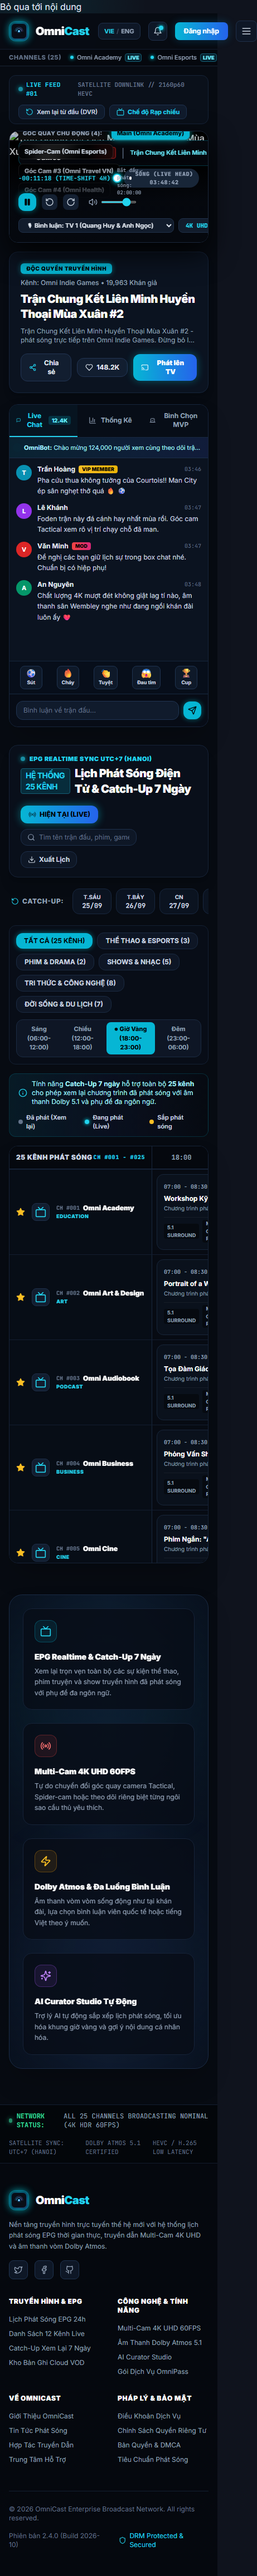
\includegraphics[width=0.6\columnwidth,height=6.5cm,keepaspectratio]{../figures/01_mobile_home.png}
\caption{\bi{Giao diện trang chủ OmniCast Mobile (\texttt{HomeScreen}): carousel sự kiện nổi bật,
thanh chuyển kênh theo thể loại và các chương trình đang/sắp phát sóng.}{The
OmniCast Mobile home view (\texttt{HomeScreen}): featured broadcast carousel, category selector,
and live/upcoming electronic programme guide.}}
\label{fig:mob_home}
\end{figure}

\subsection{\bi{Hệ thống điều hướng khai báo với GoRouter}{Declarative Routing with GoRouter}}

\bi{
Toàn bộ luồng chuyển màn hình được điều khiển bởi gói \texttt{go\_router}
thông qua mô hình khai báo tập trung trong \texttt{app\_router.dart} (Hình~\ref{fig:mob_screen_map}). Mô hình
này mang lại ba ưu thế vượt trội:
}{
The client's comprehensive routing topology is orchestrated via
\texttt{go\_router} declared centrally in \texttt{app\_router.dart} (Fig.~\ref{fig:mob_screen_map}). This
architecture unlocks three critical capabilities:
}

\begin{figure*}[t]
\centering
\fitfull{\figMobileScreenMap}
\caption{\bi{Sơ đồ kiến trúc điều hướng \texttt{GoRouter} và phân cấp 31 màn hình của OmniCast Mobile.}{Declarative \texttt{GoRouter} navigation topology and 31-screen hierarchy of OmniCast Mobile.}}
\label{fig:mob_screen_map}
\end{figure*}

\begin{enumerate}[leftmargin=*,itemsep=2pt]
  \item \textbf{\bi{Bảo vệ tuyến đường theo phiên và phân quyền RBAC:}{Auth-Guarded \& Role-Aware Routing:}}
  \bi{Khi người dùng truy cập các màn hình cá nhân hóa hoặc quản trị như \texttt{/studio/live},
  \texttt{/admin/manage} hoặc \texttt{/admin/ai-curator}, bộ định tuyến kiểm tra
  trạng thái \texttt{AuthBloc} và vai trò (\texttt{VIEWER}, \texttt{STAFF}, \texttt{ADMIN}) để bảo vệ nghiêm ngặt quyền truy cập.}{%
  Attempting to enter authenticated or role-restricted zones such as \texttt{/studio/live},
  \texttt{/admin/manage}, or \texttt{/admin/ai-curator} triggers automatic checks
  against \texttt{AuthBloc} and role permissions (\texttt{VIEWER}, \texttt{STAFF}, \texttt{ADMIN}).}

  \item \textbf{\bi{Hỗ trợ liên kết sâu (Deep Linking):}{Deep-Linking Support:}}
  \bi{Hỗ trợ phân giải các đường dẫn như \texttt{/live/:id}, \texttt{/channels/:id}, \texttt{/programs/:id} và \texttt{/recordings/:id}, cho phép mở chính xác màn hình chi tiết sự
  kiện từ các thông báo đẩy FCM hoặc liên kết chia sẻ.}{%
  Natively maps routes such as \texttt{/live/:id}, \texttt{/channels/:id}, \texttt{/programs/:id} and \texttt{/recordings/:id}, routing users directly to destination views
  from FCM push alerts or shared links.}

  \item \textbf{\bi{Khung điều hướng 6 Tab (\texttt{MainNavigationShell}):}{6-Tab \texttt{MainNavigationShell}:}}
  \bi{\texttt{ShellRoute} quản lý 6 nhánh chính (\texttt{/home}, \texttt{/channels}, \texttt{/schedule}, \texttt{/saved}, \texttt{/history}, \texttt{/profile}), duy trì trạng thái mượt mà khi chuyển
  đổi qua lại giữa các tab.}{%
  A \texttt{ShellRoute} governing 6 primary destinations (\texttt{/home}, \texttt{/channels}, \texttt{/schedule}, \texttt{/saved}, \texttt{/history}, \texttt{/profile}) preserves navigation context across tab switches.}
\end{enumerate}

\subsection{\bi{Danh mục đầy đủ 31 Màn hình Ứng dụng Di động}{Complete Inventory of All 31 Mobile Application Screens}}

\bi{
Bảng~\ref{tab:mob_screens} liệt kê toàn bộ 31 tệp màn hình thực tế trong \texttt{mobile/lib/presentation/screens/} được phân chia thành 5 cụm nghiệp vụ:
}{
Table~\ref{tab:mob_screens} catalogues all 31 concrete screen implementations under \texttt{mobile/lib/presentation/screens/} across 5 operational clusters:
}

\begin{table*}[t]
\caption{\bi{Danh mục toàn bộ 31 Màn hình trong Ứng dụng Di động OmniCast Mobile (\texttt{mobile/lib/presentation/screens/}).}{Complete inventory of all 31 screens in OmniCast Mobile (\texttt{mobile/lib/presentation/screens/}).}}
\label{tab:mob_screens}
\centering
\scriptsize
\begin{tabular}{@{}p{2.9cm}p{4.3cm}p{1.6cm}p{8.0cm}@{}}
\toprule
\textbf{\bi{Cụm chức năng}{Cluster}} & \textbf{\bi{Tệp màn hình \& Lớp (31)}{Screen Class \& Route (31)}} & \textbf{\bi{Phân quyền}{RBAC Role}} & \textbf{\bi{Tính năng \& Thao tác màn hình chính}{Key Screen Features \& Interactive Operations}} \\
\midrule
\multirow{3}{2.9cm}{\textbf{\bi{1. Khởi động \& Xác thực (6)}{1. Onboarding \& Auth (6)}}}
  & \texttt{SplashScreen} (\texttt{/}), \texttt{OnboardingScreen} (\texttt{/onboarding}) & Public & \bi{Kiểm tra phiên JWT lưu trong Secure Storage, giới thiệu tính năng lần đầu mở ứng dụng.}{JWT session check via Secure Storage, interactive first-launch onboarding tour.} \\
  & \texttt{LoginScreen} (\texttt{/login}), \texttt{RegisterScreen} (\texttt{/register}) & Public & \bi{Đăng nhập Email/Mật khẩu + Google Sign-In, đăng ký tài khoản có kiểm tra độ mạnh mật khẩu.}{Email/Password + Google Sign-In, account registration with password strength validation.} \\
  & \texttt{ForgotPasswordScreen}, \texttt{ResetPasswordScreen} & Public & \bi{Gửi mã khôi phục mật khẩu qua email và đặt lại mật khẩu mới bằng mã token 6 số.}{Request password reset token via email and set new password using a 6-digit code.} \\
\midrule
\multirow{5}{2.9cm}{\textbf{\bi{2. Khám phá \& Lịch phát EPG (8)}{2. Discovery \& EPG (8)}}}
  & \texttt{MainNavigationShell}, \texttt{HomeScreen} (\texttt{/home}) & Public / Viewer & \bi{Khung điều hướng 6 tab, carousel sự kiện đang LIVE, kênh nổi bật, tiếp tục xem và chương trình đề xuất.}{6-tab navigation shell, LIVE spotlight carousel, featured channels, continue watching and curated picks.} \\
  & \texttt{ChannelsScreen} (\texttt{/channels}), \texttt{ChannelDetailScreen} (\texttt{/channels/:id}) & Public / Viewer & \bi{Danh mục kênh lọc theo thể loại, trang chi tiết kênh phát trực tiếp bằng \texttt{OmniPlayer}, theo dõi kênh \& lịch phát.}{Category-filtered channel directory, channel detail view with embedded \texttt{OmniPlayer}, follow toggle \& EPG.} \\
  & \texttt{ScheduleScreen} (\texttt{/schedule}), \texttt{ProgramDetailScreen} (\texttt{/programs/:id}) & Public / Viewer & \bi{Lưới lịch phát điện tử EPG 24/7 hỗ trợ ngoại tuyến SQLite, chi tiết chương trình, thẻ sản xuất \& đặt hẹn nhắc 15 phút.}{Offline-capable 24/7 EPG timeline grid, programme detail view, production tags \& 15-min local alarm reminder.} \\
  & \texttt{SearchScreen} (\texttt{/search}), \texttt{CategoryBrowseScreen} (\texttt{/categories}) & Public / Viewer & \bi{Tìm kiếm liên thực thể có chống dội (\texttt{restartable} debounce) và duyệt kho nội dung theo từng chuyên mục.}{Debounced cross-entity search (\texttt{restartable} BLoC transformer) and category browser.} \\
\midrule
\multirow{3}{2.9cm}{\textbf{\bi{3. Phòng Xem LiveStream \& VOD (3)}{3. LiveStream \& VOD (3)}}}
  & \texttt{LiveNowScreen} (\texttt{/live}) & Public / Viewer & \bi{Trung tâm Đang Phát Sóng: tự động làm mới 15s, thống kê tổng sự kiện LIVE \& tổng mắt xem CCU, sắp xếp nóng/mới nhất.}{Live Broadcast Hub: 15s auto-refresh, total LIVE events \& aggregate CCU pills, trending/newest sort.} \\
  & \texttt{LiveWatchScreen} (\texttt{/live/:id}) & Public / Viewer & \bi{Phòng xem LiveStream tương tác: Sảnh chờ \texttt{LiveJoinPromptBanner}, \texttt{OmniPlayer} tự quét LAN IP, Chat phân nhánh, Biểu cảm nổi 0ms Haptic, Super Chat 6 mệnh giá (\texttt{LiveDonationModal}), Thông báo ghim từ Host \& Đổi chương trình tức thời.}{Interactive Live Watch Room: \texttt{LiveJoinPromptBanner}, LAN-aware \texttt{OmniPlayer}, threaded live chat, 0ms haptic floating reactions, 6-tier Super Chat (\texttt{LiveDonationModal}), pinned host banner \& on-the-fly program switch.} \\
  & \texttt{RecordingWatchScreen} (\texttt{/recordings/:id}) & Public / Viewer & \bi{Màn hình xem lại bản ghi VOD đa luồng, tự động lưu vị trí đang xem, bình luận phân nhánh và gợi ý video liên quan.}{VOD recording playback screen, resume-position tracking, threaded comments and related recordings.} \\
\midrule
\multirow{3}{2.9cm}{\textbf{\bi{4. Bàn điều khiển Studio \& Quản trị (5)}{4. Studio \& Admin (5)}}}
  & \texttt{LiveStudioScreen} (\texttt{/studio/live}) & \texttt{STAFF}+ & \bi{Bàn điều khiển phát sóng 4 Tab: (1) Chọn VOD lên sóng; (2) Tự ghi hình / Upload Cloudinary có chữ ký; (3) Kho công khai; (4) Thông báo ghim \& Dừng sóng.}{4-Tab Mobile Broadcast Console: (1) Curated VOD Live; (2) Self-Record / Signed Cloudinary Upload; (3) Public Catalog; (4) Host Announcement \& Stop Live.} \\
  & \texttt{MobileStudioRecorderScreen} & \texttt{STAFF}+ & \bi{Máy quay hiện trường: Đẩy sóng trực tiếp WebRTC WHIP (\texttt{Push-to-Live}) hoặc Ghi 1080p (\texttt{Record-then-Live}), mã SMPTE Timecode, Stereo VU Meter, Teleprompter HUD, lưới Rule-of-Thirds \& duyệt Master QC.}{Field Reporter Viewfinder: real-time WebRTC WHIP (\texttt{Push-to-Live}) or 1080p MP4 (\texttt{Record-then-Live}), SMPTE timecode, Stereo VU meter, Teleprompter HUD, Rule-of-Thirds \& Master QC review.} \\
  & \texttt{AdminManageScreen} (\texttt{/admin/manage}), \texttt{ScheduleFormScreen}, \texttt{AiCuratorScreen} & \texttt{STAFF}+ / \texttt{ADMIN} & \bi{Trung tâm quản trị 4 tab (Kênh, Chương trình, Lịch phát, Người dùng), biểu mẫu kiểm tra xung đột lịch EPG và bàn làm việc AI Curator.}{4-tab Admin Hub (Channels, Programmes, Schedules, Users), EPG conflict-checked schedule form and AI Curator workbench.} \\
\midrule
\multirow{4}{2.9cm}{\textbf{\bi{5. Cá nhân, Ngoại tuyến \& Pháp lý (9)}{5. Personal, Offline \& Legal (9)}}}
  & \texttt{WatchlistScreen} (\texttt{/saved}), \texttt{WatchHistoryScreen} (\texttt{/history}) & \texttt{VIEWER}+ & \bi{Danh sách theo dõi đồng bộ ngoại tuyến SQLite (\texttt{pending\_ops}), lọc theo trạng thái và lịch sử xem kèm thanh tiến độ.}{Offline-first SQLite watchlist (\texttt{pending\_ops}), status filter chips and watch history with progress bars.} \\
  & \texttt{NotificationsScreen}, \texttt{ProfileScreen}, \texttt{EditProfileScreen}, \texttt{SubscriptionPlansScreen} & \texttt{VIEWER}+ & \bi{Trung tâm thông báo FCM/Local, hồ sơ cá nhân, chỉnh sửa ảnh đại diện và đăng ký/nâng cấp gói VIP.}{FCM/Local notification centre, user profile, avatar editor and VIP subscription plan checkout.} \\
  & \texttt{SettingsScreen}, \texttt{BroadcastStandardsScreen}, \texttt{LegalDocumentScreen} & Public / Viewer & \bi{Cài đặt giao diện Sáng/Tối, ngôn ngữ Việt/Anh, cấu hình IP máy chủ, tiêu chuẩn phát sóng và văn bản pháp lý.}{Dark/Light theme toggle, VI/EN language switch, server IP config, broadcast standards and legal documents.} \\
\bottomrule
\end{tabular}
\end{table*}

\begin{figure}[t]
\centering
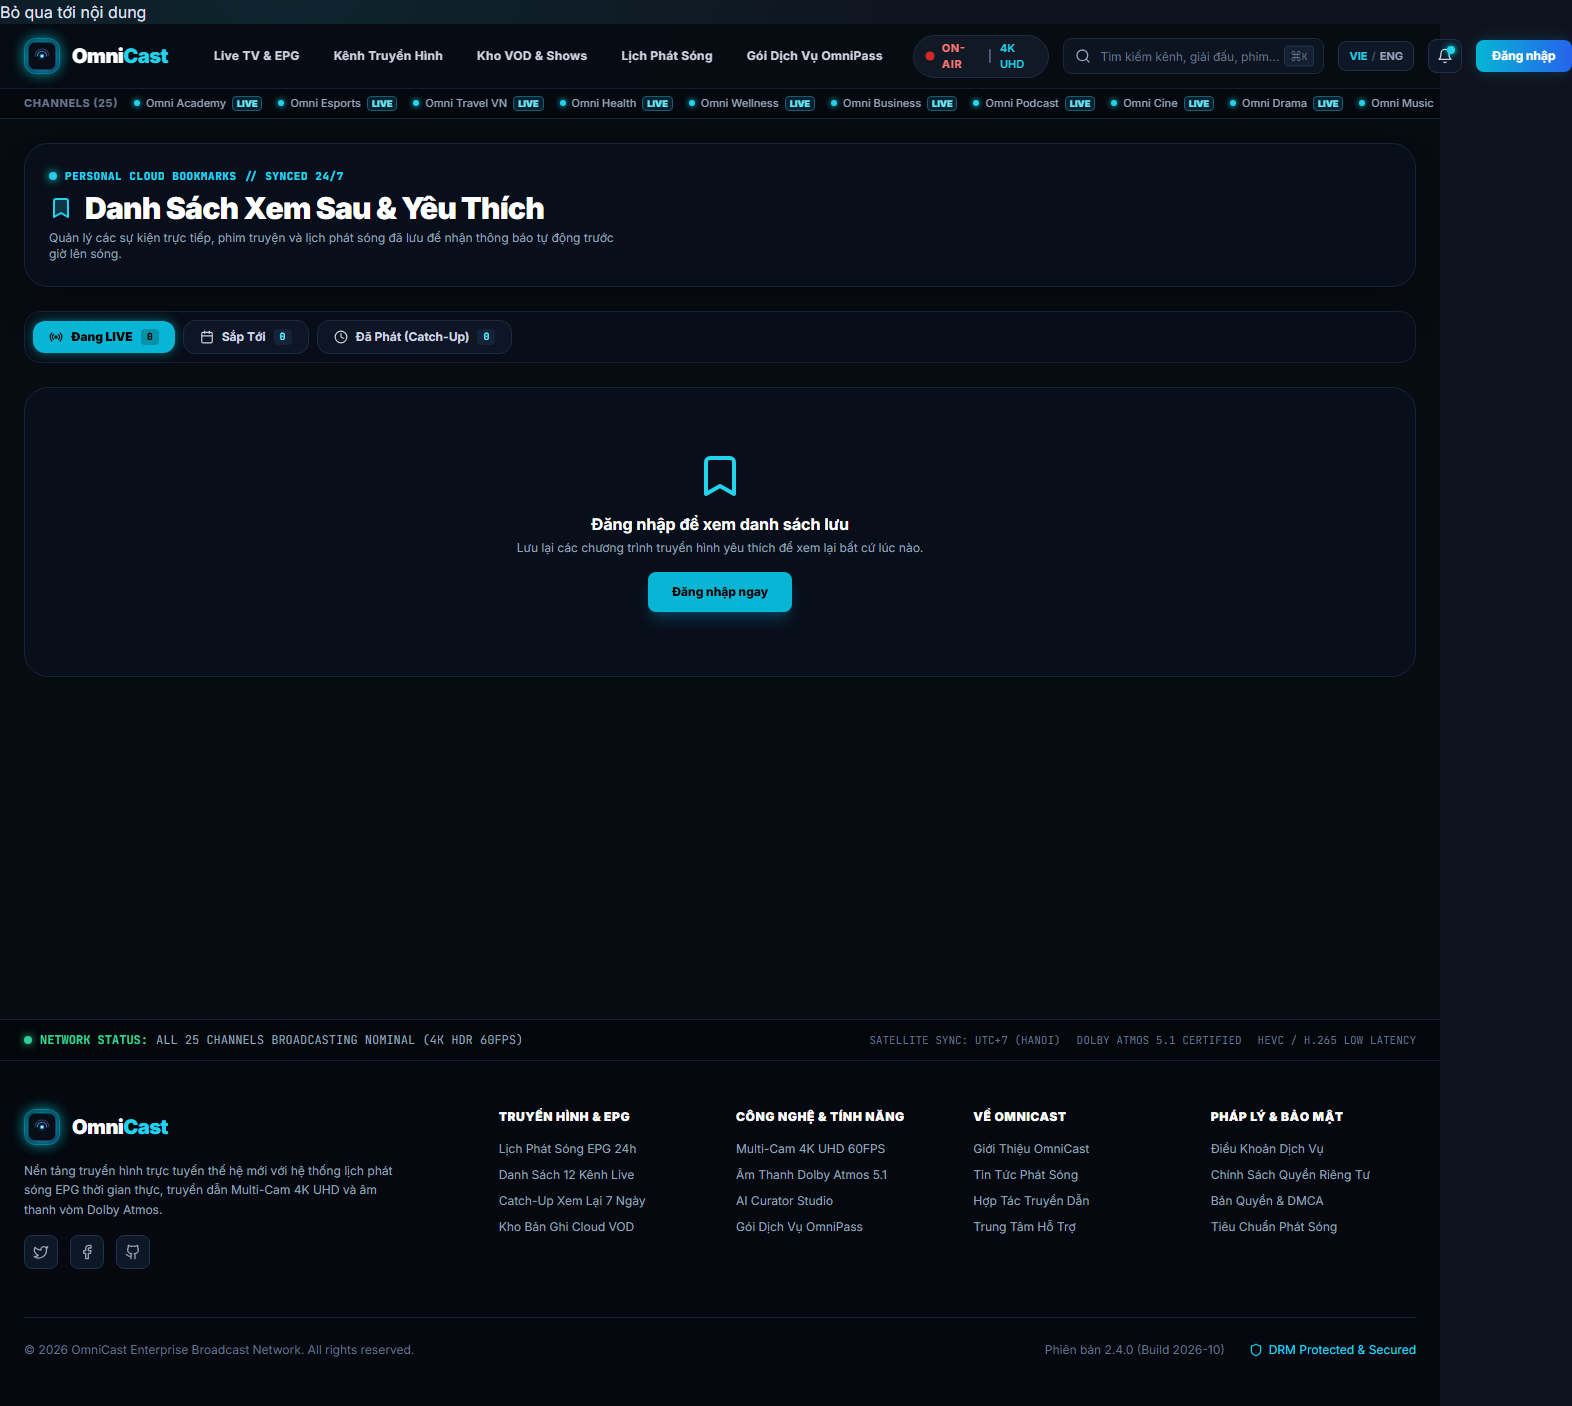
\includegraphics[width=0.48\columnwidth,height=5.2cm,keepaspectratio]{../figures/02_watchlist_screen.png}
\hfill
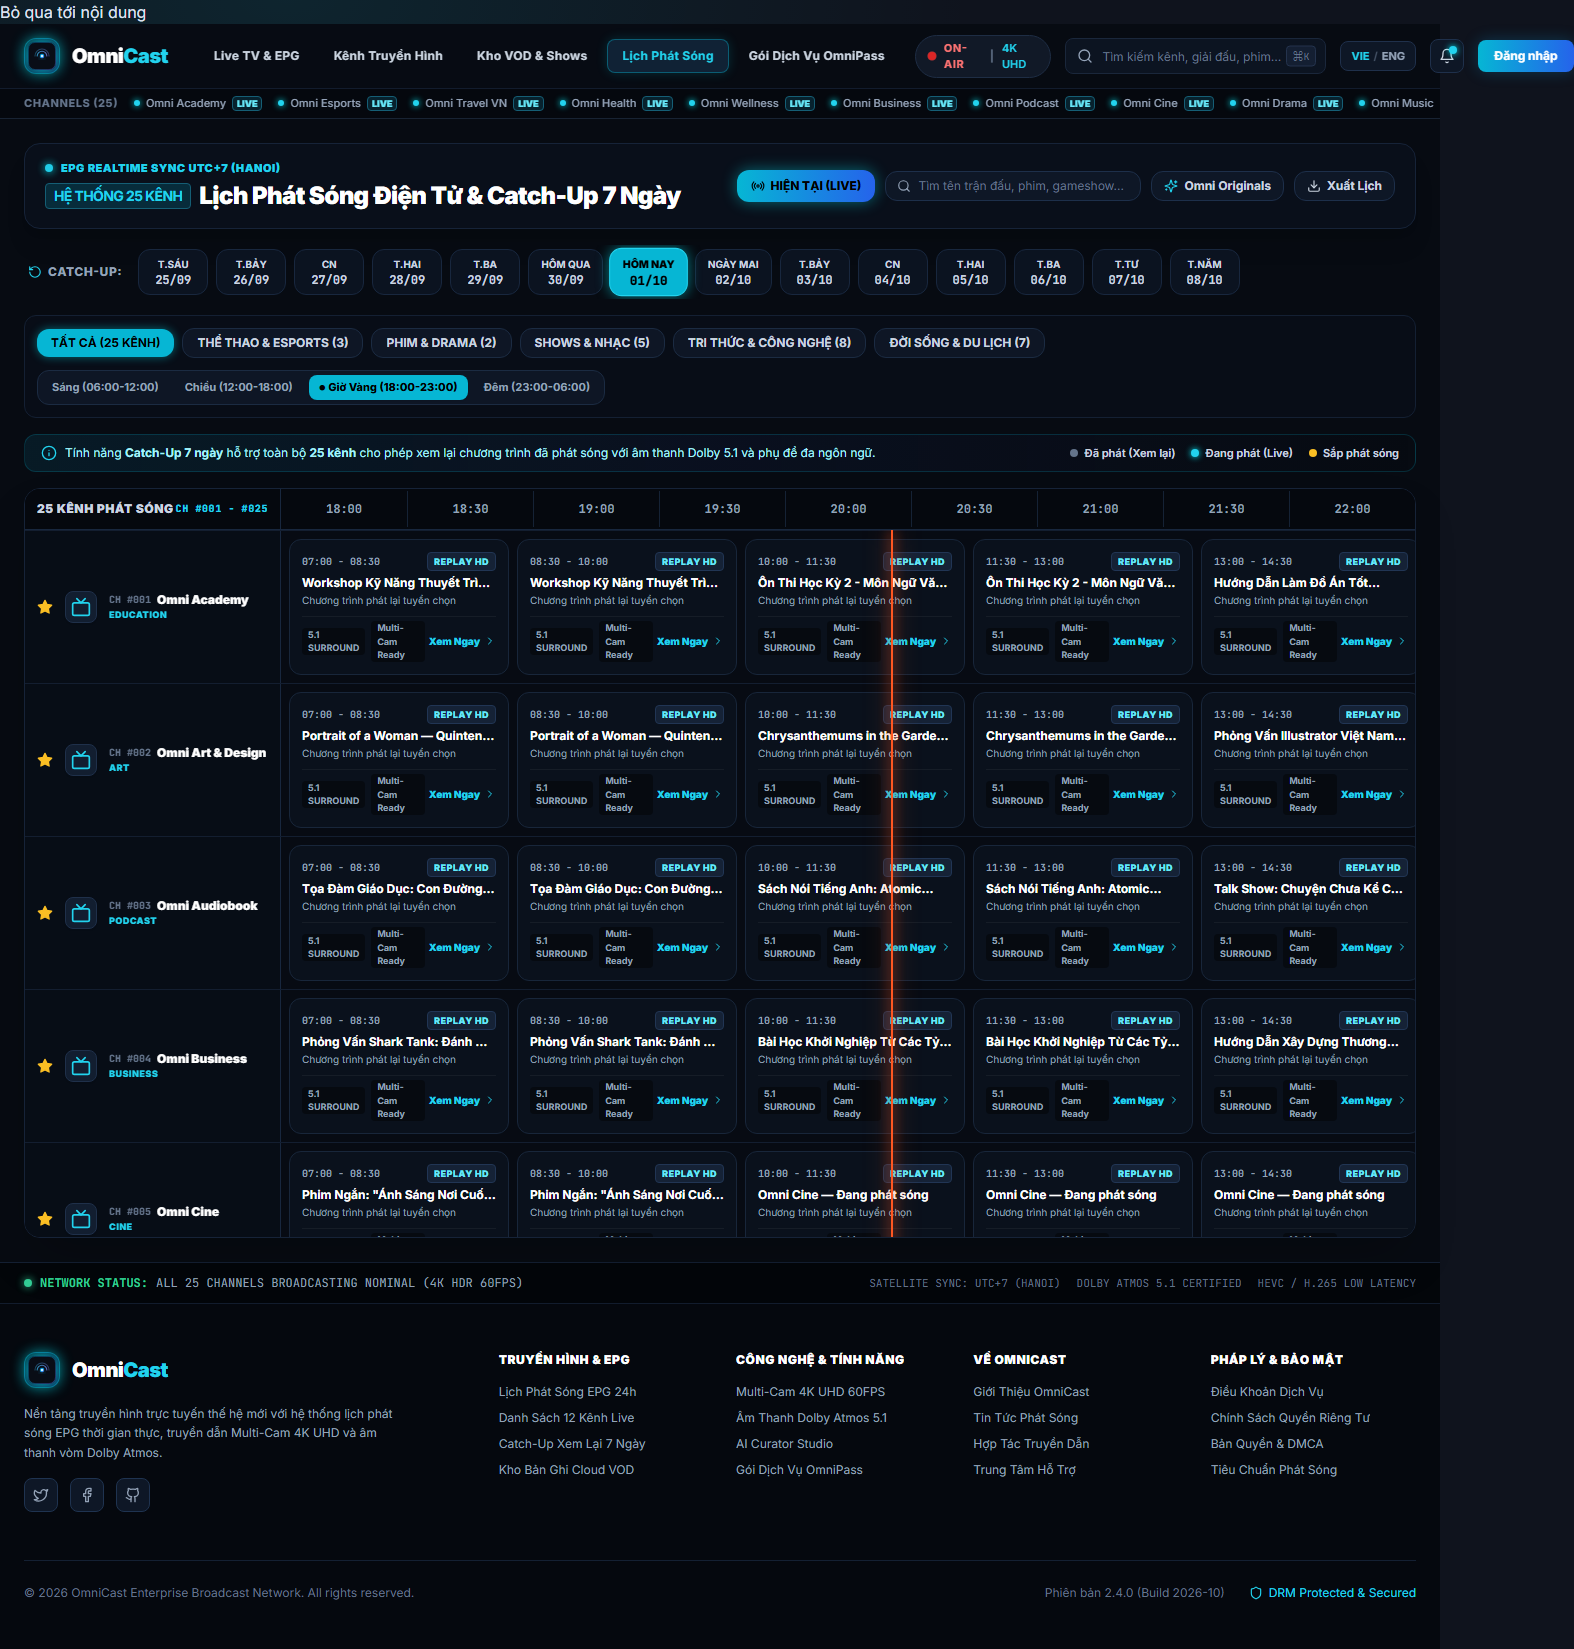
\includegraphics[width=0.48\columnwidth,height=5.2cm,keepaspectratio]{../figures/03_epg_screen.png}
\caption{\bi{Giao diện Danh sách theo dõi hỗ trợ lọc ngoại tuyến (trái) và
Lưới phát sóng điện tử EPG theo dòng thời gian 24/7 (phải).}{Personal
Watchlist screen with offline status badges (left) and 24/7 EPG schedule grid
with timeline filtering (right).}}
\label{fig:mob_subscreens}
\end{figure}
